\chapter{Weiterführenede Techniken}
\label{cha:weitere_techniken}
%
%
\section{Variieren der Interpolierungsfunktion}
\label{sec:var_der_interpolierungsfunktion}
%
Die oben aufgezeigte Interpolierungsfunktion ist in den meisten Anwendungsfällen nicht geeignet. Betrachten wir eine Figur, welche ihren Arm hebt. Zwei Keyframes wurden definiert: Die Figur mit gesenktem Arm und mit gehobenem Arm. Spielen wir dieser Animation als Schleife ab, hebt und senkt die Figur ihren Arm wiederholt. Jedoch kommt es dabei zu abrupten Richtungswechseln, welche unnatürlich wirken. Das liegt daran, dass sich physikalische Objekte nach dem Gesetz der Trägheit bewegen. Um eine Veränderung der Bewegungsrichtung zu erreichen, muss das Objekt beschleunigt werden.\newline\newline
Um diese Eigenschaft physikalischer Objekte zu simulieren, bedarf es einer Interpolierungsfunktion, wessen Ableitung keine Sprünge macht, weder zwischen zwei Keyframes noch über angrenzende Keyframes hinweg. \newline\newline
%
Die wie folgt beschriebene Funktion $ease\_in\_out$ hat diese Eigenschaften. Sie lässt die Animation langsam beginnen, dann schneller werden und zum Ende wieder langsamer werden. (vgl. \cite{Febucci2018}). Die Funktion $lerp$ wird unverändert aus Formel 2.1 übernommen:
%
\begin{equation}
	ease\_in(x) = x^2
\end{equation}
\begin{equation}
	ease\_out(x) = (1-x)^2
\end{equation}
\begin{equation}
	ease\_in\_out(x) = lerp(ease\_in(x), ease\_out(x), x)
\end{equation}
\newline
Das Ergebnis von $ease\_in\_out(x)$ setzen wir statt x in $lerp$ ein
%
\begin{equation}
	lerp(a,b,ease\_in\_out(x))
\end{equation}
%
Und bekommen somit für jeden Zeitpunkt $t$ den richtigen Transformations-Wert.
%
\section{Animation Layering}
%
Besonders in interaktiven Anwendungen ist kann es hilfreich sein, mehrere Animationen zu kombinieren. Erstellt man eine Animation für einen bestimmten Bereich, dann kann man diesen Bereich unabhängig vom Rest des Körpers animieren. Die Transformations-Werte aller betroffenen Gelenke werden je Keyframe abgespeichert. Diese werden interpoliert, um für jeden Frame wie weiter oben geschildert mit Forward Kinematics die globalen Transformations-Werte zu berechnen. Beim Animation Layering ersezt eine Ebene für den betroffen Bereich alle berechneten Werte darunterliegender Ebenen.
\newline\newline
Betrachten wir folgendes Beispiel: \newline
Zu animierende Figur hat 2 Animationen: Gehen und Winken. Die Gehen-Animation betrifft alle Gelenke der Figur. Die Winken-Animation hingegen betrifft nur die Gelenke des rechten Arms. Um beide Animationen zu kombinieren, werden die Rotationen der Armgelenke der Gehen-Animation durch die Rotationen der Winken-Animationen ersetzt.
%
\section{Additive Animation Blending}
%
Neben dem Animation Layering gibt es auch die Technik des ``Additive Animation Blending''. Zwei oder mehr Animationen werden zu einer neuen Animation zusammengefügt. Die neue Animation besteht zu vom Animator festgelegten Gewichtungen aus bereits vorhandenen Animationen. So ließe sich z.B. eine Gehen-Animation und eine Rennen-Animation kombinieren. 
%
\section{Meshes}
%
Ein Mesh(engl.: Netz) ist eine Ansammlung von Punkten und Dreiecken, welche sich aus den Verbindungslinien jeweils 3 dieser Punkte bilden. Ein solches Mesh kann als ein Array von Vertices(Punkte im Koordinatensystem) und ein Array von Indices definiert werden. Drei dieser Indices, welche auf je einen Punkt des ersten Arrays verweisen, bilden jeweils ein Dreieck. Mithilfe eines solchen Meshs können wir nun eine Textur aufspannen. Dazu definieren wir zusätlich ein Array von UVs(Bildkoordinaten). Je Punkt wird ein UV festgelegt. Unabhängig von den Koordinaten eines Punkts können wir ihm jetzt eine Position in der Textur-Bilddatei zuweisen. Mit den gegebenen Informationen kann nun die Farbe jedes Pixels innerhalb eines Dreiecks bestimmt werden. Dazu wenden wir den <<Triangle rendering algorithm>> an.
\newline\newline
Die Verwendung von Meshes zum Rendern von Grafiken bringt einige Vorteile mit sich, darunter: 
\newline
1) Bilder können nicht nur in ihrer ursprünlichen Erscheinung sondern auch in verzerrter Form angezeigt werden.
\newline
2) Transparente Bereiche von Bilddateien mit Alpha-Kanal können beim anzeichnen ignoriert werden, was die Effizienz erhöht.
%
\subsection{Mesh Generierung}
%
Je nach Verwendungszweck unterscheidet sich die Natur des am besten geeigneten Meshs. Es gilt die Größe der vom Mesh bedeckten Fläche zu minimieren, um die Effizienz zu maximieren. Das bedeutet, das Mesh sollte alle sichtbaren Bereiche bedecken, damit diese vollständig angezeigt werden, aber vollständig transparente Bereiche sollten möglichst ausgelassen werden.\newline
\newline
Die Dichte von Dreiecken in einem Bereich des Bildes und die Form und Lage der Dreiecke beeinflusst die Art und Weise, auf welche sich die angezeigte Grafik bei Verzerrung des Meshs verändert. Übermäßig große Dreiecke, besonders in Bereichen, welche stark verzerrt werden, führen meist zu einem unnatürlich erscheinendem Ergebnis.
%
\subsubsection{Marching Squares Algorithmus}
Um ein enganliegendes Mesh zu generieren, berechnen wir erst einmal eine Kontur für unsere Bilddatei, in unserem Fall ein Bild im PNG-Format. Um aus einer Bilddatei eine Kontur zu generieren, kann der Marching Squares Algorithmus (engl.: wandernde Quadrate) angewandt werden. Die Kontur sollte etwas weiter als die tatsächliche Kontur des abgebildeten Objekts sein. Das dient dazu, dass alle sichtbaren Teile beim Rendern später vollständig gezeichnet werden. Zudem ermöglicht es das aussortieren überflüssiger Eckpunkte, die durch den Marching Squares Algorithmus entstehen. (vgl. \cite{Maple2003})\newline\newline

Unser Ziel ist es, eine Kontur um alle sichtbaren Teile der Bilddatei zu ziehen. Als sichtbar sehen wir alles an, was einen festgelegten Alpha-Schwellwert überschreitet. Dazu generieren wir aus dem Alpha-Kanal des Bildes ein Distanzfeld. Das Distanzfeld ist eine Grauwertmatrix der selben Auflösung des Bildes. Für jeden Pixel der Bilddatei wird hier die Distanz zum nächstgelegenen sichtbaren Pixel berechnet und festgehalten. Anhand eines weiteren Schwellwerts generieren wir ein Raster, dessen Zellen jeweils entweder $true$ für sichtbar oder $false$ für unsichtbar sind.
Auf dieses Raster wird nun ein Konturraster gelegt, welches in x- und y-Richtung jeweils eine Zelle kleiner ist. Die Eckpunkte des Konturrasters liegen jeweils im Zentrum einer der Binärzellen. Jeder Zelle des Konturrasters wird ein Wert zugewiesen. Dieser ergibt sich daraus, ob die Werte der vier Ecken dieser Zelle $true$ oder $false$ sind. Den Ecken werden die Werte $2^0$, $2^1$, $2^3$ und $2^4$ zugewiesen. (siehe Abb.: \ref{fig:marching_square_corners})
\cite{Wisq2022}
\begin{figure}[!htb]
	\minipage{0.3\textwidth}
	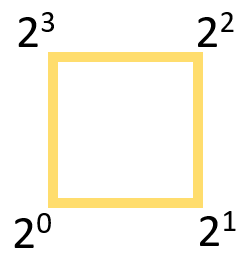
\includegraphics[width=\linewidth]{img/marching_square_corners.png}
	\caption{Konturzelle}\label{fig:marching_square_corners}
	\endminipage\hfill
	\minipage{0.5\textwidth}
	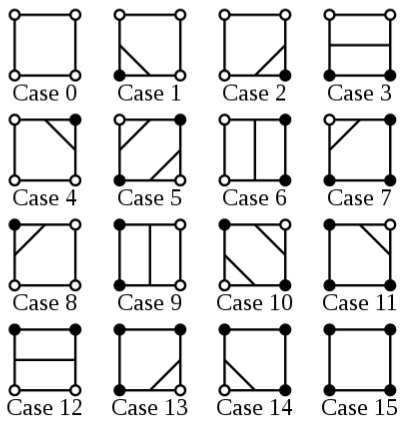
\includegraphics[width=\linewidth]{img/marching_square_wiki.png}
	\caption{Mögliche Fälle (vgl. \cite{Wisq2022	})}\label{fig:marching_square_cases}
	\endminipage\hfill
\end{figure}
%
Für jede der 15 möglichen Kombinationen wird jeweils ein entsprechendes Konturstück festgelegt. Diese 15 Fälle können in einer Lookup-Tabelle gespeichert werden. Fügt man all diese Stücke zusammen ergibt sich die gesuchte Kontur. Abb. \ref{fig:marching_square_example} und \ref{fig:marching_square_example_solved} zeigen die Vorgangsweise an einem Beispiel.
\begin{figure}[!htb]
	\minipage{0.4\textwidth}
	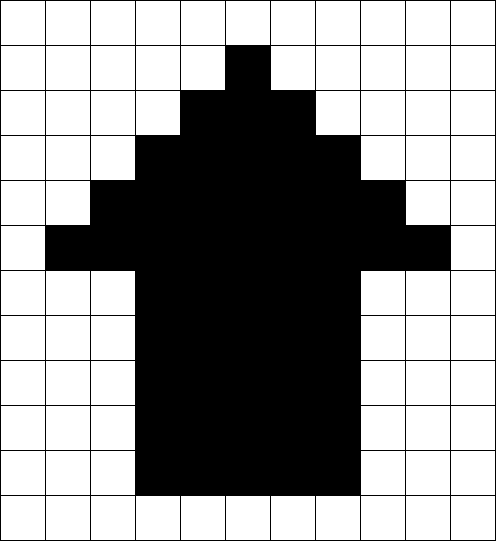
\includegraphics[width=\linewidth]{img/marching_square_example.png}
	\caption{Ausgangsposition}\label{fig:marching_square_example}
	\endminipage\hfill
	\minipage{0.4\textwidth}
	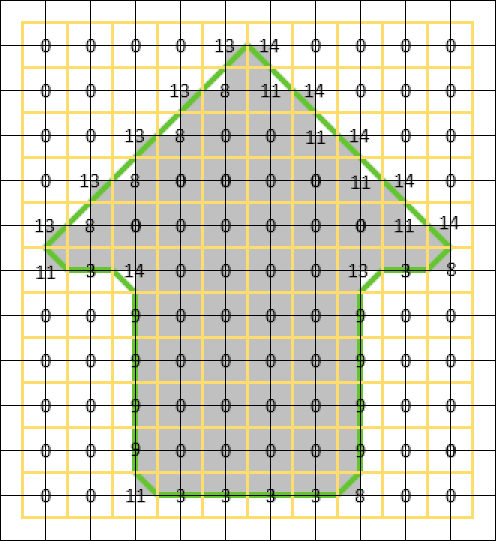
\includegraphics[width=\linewidth]{img/marching_square_example_solved.png}
	\caption{Zielposition}\label{fig:marching_square_example_solved}
	\endminipage\hfill
\end{figure}
%
Wir generieren nun aus den Zellen einen ungerichteten Graphen.
%
\subsection{Mesh Deformierung}
Die Deformierung des Meshs erfolgt durch die Verschiebung der dazugehörigen Punkte. Um eine solche Deformierung durch das Transformieren der Skelett-Knochen zu erreichen, legen wir den Einflussgrad jedes Knochens auf jeden Mesh-Punkt fest. Zusätzlich legen wir die Lage jedes Punktes relativ zur Lage, Rotation und Skalierung jedes auf ihn Einfluss nehmenden Knochens fest. Für jeden Mesh-Punkt ergeben sich nun bei beliebiger Skelettpose eine Anzahl an globalen Koordinaten. Die endgültige Punktkoordinate ergibt sich zu festgelegten Anteielen aus diesen global Koordinaten. Das angepasste Mesh geben wir an die Graphics Library weiter, welche sich um das Rendern kümmert.
%
\section{Prozedurale Animation}
Oft ist es von Vorteil, wenn Teile einer Animation nicht direkt vom Animator gestaltet werden müssen, sondern prozedural erstellt werden. Soll zum Beispiel eine humanoide Figur mit der Hand nach einem Objekt greifen, ist es mühselig und zeitaufwendig jeden Abschnitt des Arms einzeln zu animieren. Inverse Kinematics machen es möglich mittels der Position und Orientierung der Hand auf die Position und Rotation aller Armabschnitte zu schließen. Dies Bedarf keiner weiteren Eingabe des Animators.\newline\newline
Ein weiteres Beispiel für prozedurale Animation ist Physik-Simulation. Die automatische Animierung von Objekten, welche sich nach grundlegenden physikalischen Gesetzen verhalten, spart Zeit. Darüber hinaus ist sie meist genauer, als die Animierung von Hand. Ein Anwendungsfall für Physik-Simulation ist ein herabhängendes Stück Stoff, das von einer Person getragen wird.\newline\newline
Ein weiterer Vorteil von prozeduraler Animation ist, dass nicht alle Details zur Erstellung der Animation bekannt sein müssen. So ist es z.B. möglich, dass eine animierte Figur mit der Umgebung interagiert, obwohl diese erst zu Laufzeit des Programms bekannt ist und Nutzereingaben können mit in die Animation einspielen.
%
\section{Inverse Kinematics}
%
Der Begriff „Inverse Kinematics“ (engl.: inverse Kinematik) kommt aus der Robotik. Um den Endeffektor eines Roboterarms mit n Gelenken und Verbindungsstücken an gewünschte kartesische Koordinaten mit gewünschter Orientierung zu bewegen, wird ein Algorithmus benötigt. Ziel dieses Algorithmus ist die Errechnung der passenden Einstellung jedes beteiligten Gelenks.\newline\newline

Eine Kette von Gelenken und Knochen in der Skelettanimation hat die gleiche Struktur wie ein Roboterarm mit Gelenken und Verbindungsstücken. Die gleichen Techniken, welche zur Lösung von Inverse Kinematics in der Robotik eingesetzt werden, sind daher auch in der Skelettanimation anwendbar.
%
\subsection{Algebraische Methode für 2 Gelenke}
\begin{figure}[!htb]
	\minipage{0.5\textwidth}
	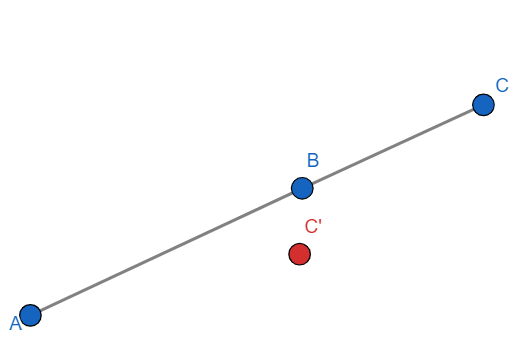
\includegraphics[width=\linewidth]{img/roboterarm_0.png}
	\caption{Ausgangsposition}\label{fig:roboterarm_0}
	\endminipage\hfill
	\minipage{0.5\textwidth}
	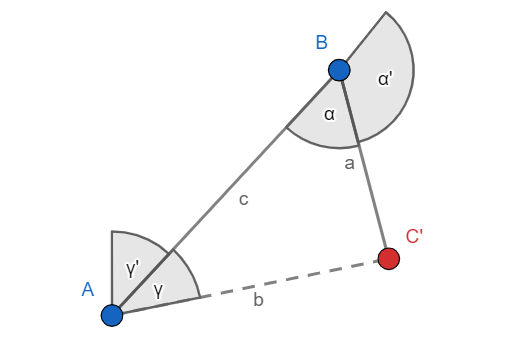
\includegraphics[width=\linewidth]{img/roboterarm_1.png}
	\caption{Zielposition}\label{fig:roboterarm_1}
	\endminipage\hfill
\end{figure}
Wir betrachten einen Roboterarm (siehe Abbildung \ref{fig:roboterarm_0}). Der Arm hat 2 Gelenke $A$ und $B$. $A$ ist fixiert. Am Ende des Arms ist der Endeffektor $C$ befestigt. Nun soll $C$ zur Zielposition $C'$ bewegt werden. Dieses Problem kann mit dem Gesetz des Kosinus gelöst werden. Abbildung \ref{fig:roboterarm_1} zeigt den Roboterarm in der Zielstellung. $a$, $b$ und $c$ bilden zusammen ein Dreieck. Mit dem Gesetz des Kosinus(Gleichung 3.1) ermitteln wir die Winkel $\gamma$ und $\alpha$.\\
\begin{equation}
	\begin{split}
		c^2=a^2+b^2-2ab \cdot cos(\theta)\\
		\theta=cos^{-1}\left(\frac{a^2+b^2-c^2}{2ab}\right)
	\end{split}
\end{equation}
\begin{equation*}
	\gamma=cos^{-1}\left(\frac{a^2+b^2-c^2}{2ab}\right)
\end{equation*}
\begin{equation*}
	\alpha=cos^{-1}\left(\frac{c^2+b^2-a^2}{2cb}\right)
\end{equation*}
Die Winkel, welche wir eigentlich brauchen sind $\gamma'$ und $\beta'$. Diese sind die benötigten Winkeleinstellungen für die jeweiligen Gelenke\footnote{Wir definieren senkrecht nach oben als den Nullwinkel und bewegen uns von hieraus im1 Uhrzeigersinn}. Wir berechnen die beiden gesuchten Winkel wie folgt:
\begin{align*}
	&\alpha' = \pi - \alpha \\
	&\gamma' = tan^{-1}\left(\frac{\vec{AC}_x}{\vec{AC}_y}\right)
\end{align*}
%
\subsection{Cyclic Coordinate Descent}
Cyclic Coordinate Descent (CCD) ist eine iterative Methode zur Lösung von Inverse Kinematics. Alle Gelenke welche Teil der betroffenen kinematischen Kette sind, werden nacheinander rotiert, um den Abstand zur Zielposition zu minimieren. Dabei werden alle Gelenke von der tiefsten bis zur höchsten Ebene in der Hierarchie abgearbeitet. Dieser Vorgang wird wiederholt bis der Endeffektor annäherungsweise die gewünschte Position erreicht hat.
\newline\newline
\begin{figure}[!htb]
	\minipage{0.5\textwidth}
	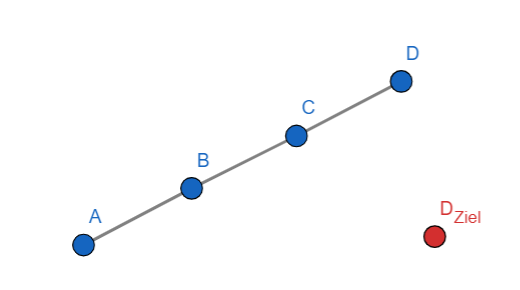
\includegraphics[width=\linewidth]{img/ccd_0.png}
	\caption{Ausgangsposition}\label{fig:ccd_0}
	\endminipage\hfill
	\minipage{0.5\textwidth}
	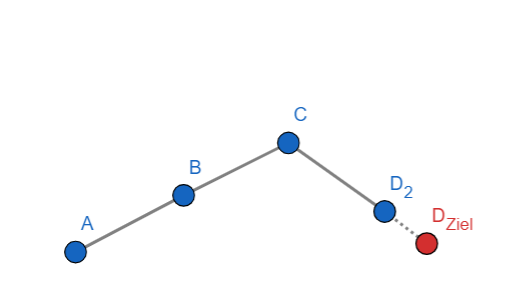
\includegraphics[width=\linewidth]{img/ccd_1.png}
	\caption{}\label{fig:ccd_1}
	\endminipage\hfill
\end{figure} 
Abbildung \ref{fig:ccd_0} zeigt einen Roboterarm, welcher aus drei Knochen und drei Gelenken besteht. $A$ ist fixiert, $D$ ist der Endeffektor und soll zu $D_Ziel$ bewegt werden. Wir beginnen mit dem Knochen auf der untersten Ebene in der Hierarchie und rotieren diesen um den Punkt $C$, sodass $D$ auf $\vec{CD}_{Ziel}$, also dem Vektor vom betroffenen Gelenk zum Zielpunkt, liegt (siehe Abbildung \ref{fig:ccd_1}). Eine Ebene weiter oben rotieren wir um den Punkt $B$ (siehe Abbildung \ref{fig:ccd_2}), dann um den Punkt $A$ (siehe Abbildung \ref{fig:ccd_3}). Wiederholen wir diese Schritte, nähert sich D mit jeder Iteration $D_{Ziel}$ an. Der Algorithmus endet, sobald der Abstand von $D$ zu $D_{Ziel}$ einen vorher festgelegten Minimalabstand unterschreitet.
\begin{figure}[!htb]
	\minipage{0.5\textwidth}
	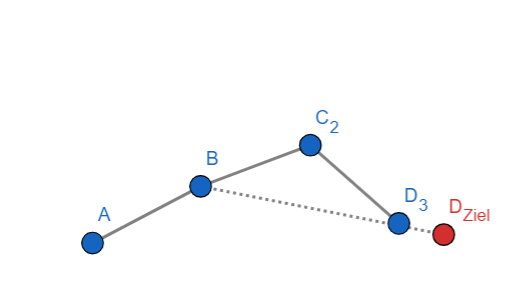
\includegraphics[width=\linewidth]{img/ccd_2.png}
	\caption{}\label{fig:ccd_2}
	\endminipage\hfill
	\minipage{0.5\textwidth}
	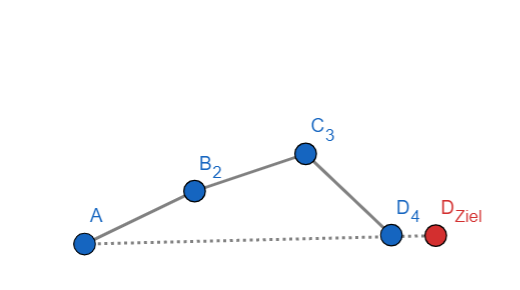
\includegraphics[width=\linewidth]{img/ccd_3.png}
	\caption{Zielposition}\label{fig:ccd_3}
	\endminipage\hfill
\end{figure}
Je nach Aufstellung kann es sein, dass viele Iterationen benötigt werden bis der Algorithmus auf diese Weise endet. Jedoch sind die Berechnungen und Transformationen nicht rechenintensiv, wodurch sich CCD für interaktive Echtzeitanwendungen eignet. (vgl. \cite{Fedor2003}: 207-208)
\subsection{Stoff-Simulation}
Eine Stück Stoff lässt sich mit Hilfe des Verlet-Algorithmus simulieren. (vgl. \cite{Counts2012}). Der Verlet-Algorithmus bestimmt die Position $x$ eines Körpers zum Zeitpunkt $t$. $v$ ist die Geschwindigkeit und $a$ die Beschleunigung des Körpers. Zur Anwendung des Verlet-Algorithmus benötigen wir zwei Positionen, $x_n$ und $x_{n-1}$. Ist die Position $x_0$ bekannt, muss zuerst die Position $x_1$ bestimmt werden. Dazu wenden wir folgende Formel an:

\begin{equation}
	\vec{x}_{1} = \vec{x}_0 + \vec{v}_{0}\Delta t + frac{1}{2} \vec{a}_0\Delta t^2 
\end{equation}

Durch Iteration des Verlet-Algorithmus können nun alle Positionen $\vec{x}_n$ bestimmt werden.

\begin{equation}
	\vec{x}_{n+1} = 2\vec{x}_n - \vec{x}_{n-1} + \vec{a}_n\Delta t^2 
\end{equation}

Es ist anzumerken, dass der Verlet-Algorithmus die Geschwindigkeitsberechnung aus der Formel für gleichmäßig beschleunigte Bewegung eliminiert. Das kommt uns zu Nutzen, da es die Stoffsimulation vereinfacht.
\newline\newline
Folgender Pseudo-Code implementiert den Verlet-Algorithmus einer Punktmasse:
\begin{adjustwidth}{1cm}{-5cm}
\begin{verbatim}
	// Compute velocity from current position - lastPosition
	velocity = position - last_position;
	
	// Save position for next frame;
	last_position = position;
	
	// Find next position
	position = position + velocity *  + (1/2 * acceleration * deltaTime);
	
	// Set acceleration to gravity
	acceleration = vector(0., -9.81, 0.);
\end{verbatim}	
\end{adjustwidth}


vgl. \cite{Wiver2022}

Wir definieren unser Stück Stoff als eine Ansammlung von Punktmassen, welche mit Gliedern verbunden sind. Eine Punktmasse ist ein Objekt ohne Ausdehnung. Es hat lediglich eine Masse und eine Position. Die Glieder werden in Beziehung zu den jeweils zwei dazugehörigen Punktmassen definiert. Die Länge eines Glieds ist der Abstand der beiden Punktmassen zueinander. Wir legen nun Constrainsts\footnote{engl. für Einschränkung, Als Constraint bezeichnen wir Bedingung z.B. den minimalen Abstand eines Objekts zu einem anderen.} für unser Stoffstück fest: Jedes Glied hat eine Soll-Länge, welche angestrebt wird.\newline\newline
Durch den Einfluss von Schwerkraft und anderen Kräften verändert sich der Abstand zwischen den Punktmassen. Um den entgegenzuwirken lösen wir die dem Stoffstück zugewiesenen Constraints\footnote{Ein Constraint wird als gelöst angesehen, wenn die ihm zugewiesene Bedingung erfüllt ist.}.\newline\newline
Ist die Distanz zwischen 2 Punktmassen, welche mit einem Glied verbunden sind, kleiner oder größer als die Soll-Länge, dann bewegen wir beide Massen aufeinander zu bzw. voneinander weg. Das tun wir nacheinander für alle Glieder. Durch das lösen eines Constraints kommt es vor, dass ein anderer Constraint den gelösten Zustand verlässt. Das führt zu einem unglaubwürdigen Verhalten des Stoffstücks, da sich einige Bereiche dehnen, während andere steiff wirken. Der Ablauf der Simulation ist zudem stark davon abhängig, welcher Constraint zuerst gelöst wird. Um diese Abweichungen zu minimieren, lösen wir die Constraints nicht nur einmal, sondern über mehrere Iterationen hinweg. Je mehr Iterationen durchgeführt werden, desto geringer ist der Fehler und desto steiffer wirkt das Stoffstück.
